\documentclass[naustrian]{scrartcl}
\usepackage[T1]{fontenc}
\usepackage[utf8]{inputenc}
\usepackage[scaled=.8]{beramono}
\usepackage{geometry}
\geometry{verbose,tmargin=3cm,bmargin=3cm,lmargin=3cm,rmargin=3cm}
\usepackage[ngerman]{babel}
\usepackage{microtype}
\usepackage[parfill]{parskip}
\usepackage{amsmath}
\usepackage{graphicx}
\usepackage{hyperref}
\usepackage{nameref}
\usepackage{float}
\usepackage{listings}
\usepackage{color}
\usepackage{fancyhdr}
\usepackage{blindtext}
\usepackage{algorithm}
\usepackage{algpseudocode}
\usepackage{esvect}

\usepackage{subcaption}

\pagestyle{fancy}
\fancyhf{}
\rhead{Sonja Biedermann 01402891}
\lhead{BUSII: Final Report}
\cfoot{\thepage}

\newcommand*{\fullref}[1]{\hyperref[{#1}]{\autoref*{#1}~\nameref*{#1}}}

\definecolor{darkgray}{rgb}{0.66, 0.66, 0.66}
\definecolor{asparagus}{rgb}{0.53, 0.66, 0.42}

\lstdefinestyle{s}{
  commentstyle=\color{darkgray},
  keywordstyle=\bfseries,
  morekeywords={},
  stringstyle=\color{asparagus},
  basicstyle=\ttfamily\footnotesize,
  breakatwhitespace=false,
  keepspaces=true,
  numbersep=5pt,
  showspaces=false,
  showstringspaces=false,
}

\lstset{style=s}

\makeatletter
\newsavebox\myboxA
\newsavebox\myboxB
\newlength\mylenA
\newcommand*\xoverline[2][0.75]{%
    \sbox{\myboxA}{$\m@th#2$}%
    \setbox\myboxB\null% Phantom box
    \ht\myboxB=\ht\myboxA%
    \dp\myboxB=\dp\myboxA%
    \wd\myboxB=#1\wd\myboxA% Scale phantom
    \sbox\myboxB{$\m@th\overline{\copy\myboxB}$}%  Overlined phantom
    \setlength\mylenA{\the\wd\myboxA}%   calc width diff
    \addtolength\mylenA{-\the\wd\myboxB}%
    \ifdim\wd\myboxB<\wd\myboxA%
       \rlap{\hskip 0.5\mylenA\usebox\myboxB}{\usebox\myboxA}%
    \else
        \hskip -0.5\mylenA\rlap{\usebox\myboxA}{\hskip 0.5\mylenA\usebox\myboxB}%
    \fi}
\makeatother

\begin{document}

\title{BUSII\\Final Report}

\author{Sonja Biedermann,\\01402891}

\maketitle

\section{Objective}

Our objective was to implement a tool that could be used like something akin
to a debugger for the machining process data. It should be possible to step
through time and see which tools were used when, where the tool was in space,
and the readings of the various sensors (e.g. load, torque).

Further, it should be possible to label sections of time where something unusual
happened, and these labels should be able to be exported for later use with e.g.
ML algorithms or other analysis tools.

\section{Prototype}

Our initial low-fidelity prototype is shown in
Figures~\ref{fig:lofi-1}~and~\ref{fig:lofi-2}.  Figure~\ref{fig:hifi} shows the
main view of the high-fidelity prototype we implemented.

The first view of the low-fidelity prototype (Figure~\ref{fig:lofi-1}) was
scrapped in favor of the more compact representation of the process tree shown
in Figure~\ref{fig:select}. This was done because it became evident that
rendering a tree in SVG would not scale to hundreds of processes.

Otherwise, the final prototype is a pretty faithful realization of the second view
of the low-fidelity prototype.

\begin{figure}
    \centering

    \begin{subfigure}{0.5\textwidth}
        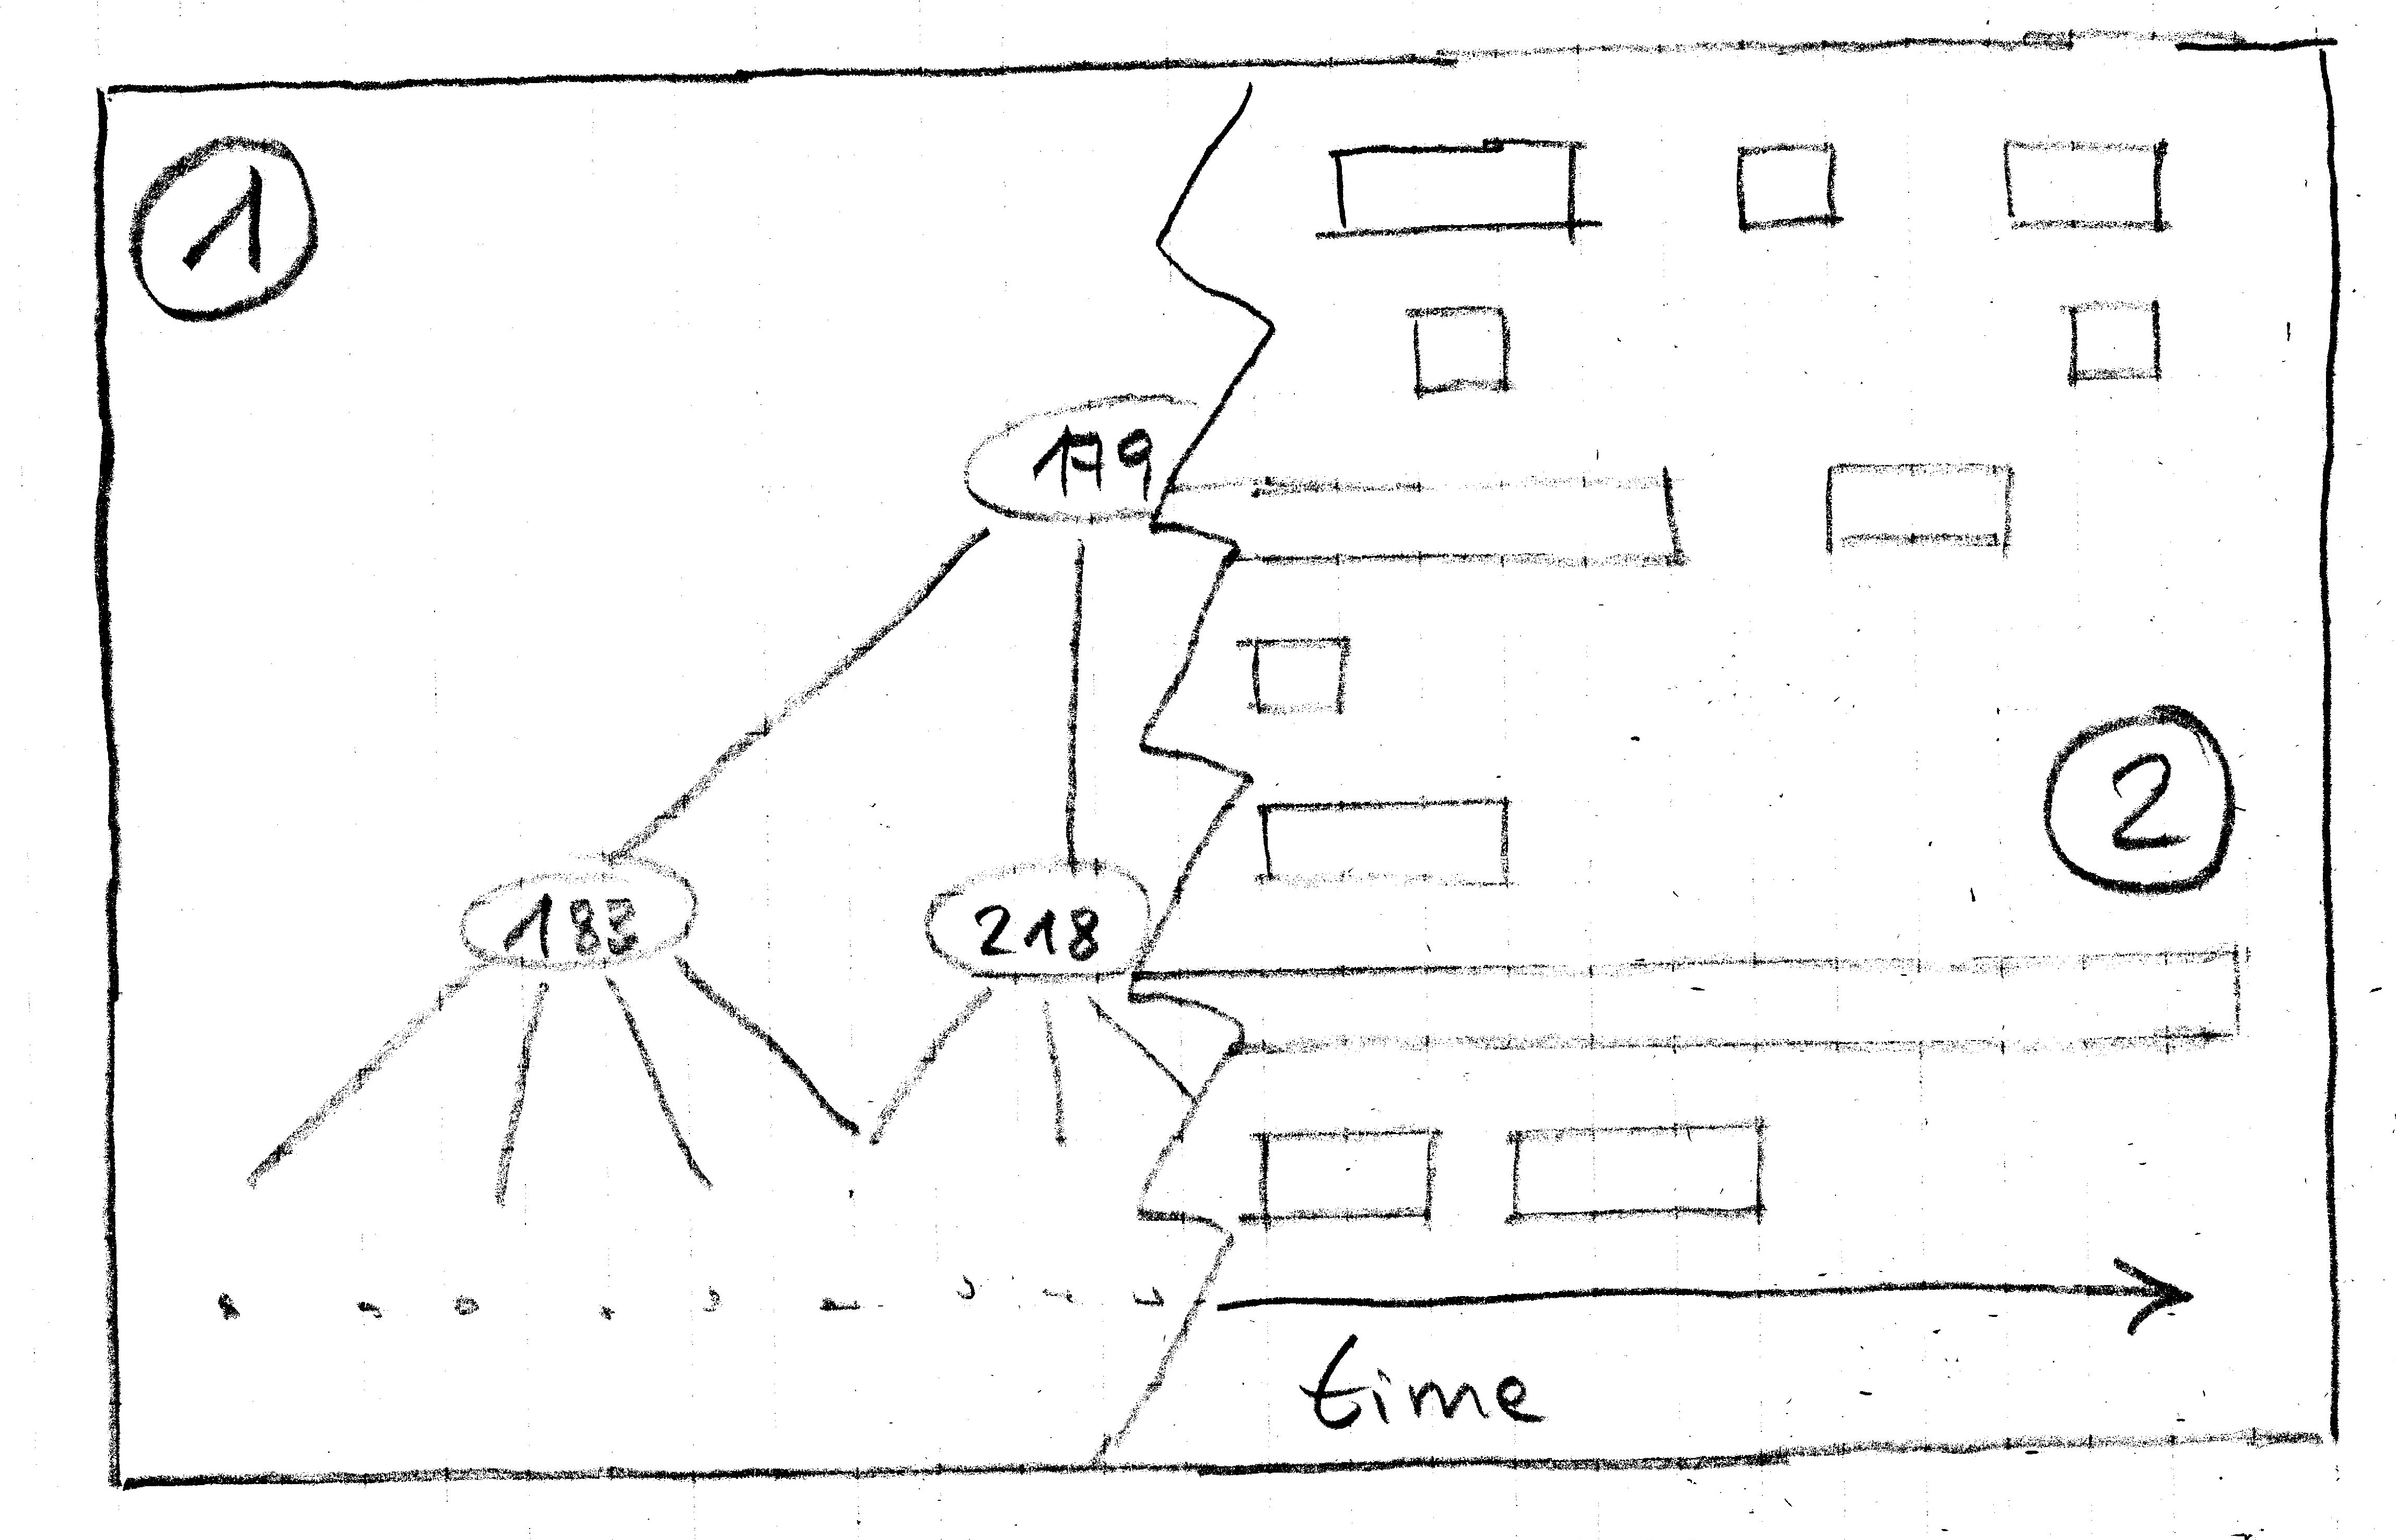
\includegraphics[width=\textwidth]{img/proto_1.jpg}
        \caption{Low-fidelity prototype view 1}
        \label{fig:lofi-1}
    \end{subfigure}%
    ~
    \begin{subfigure}{0.5\textwidth}
        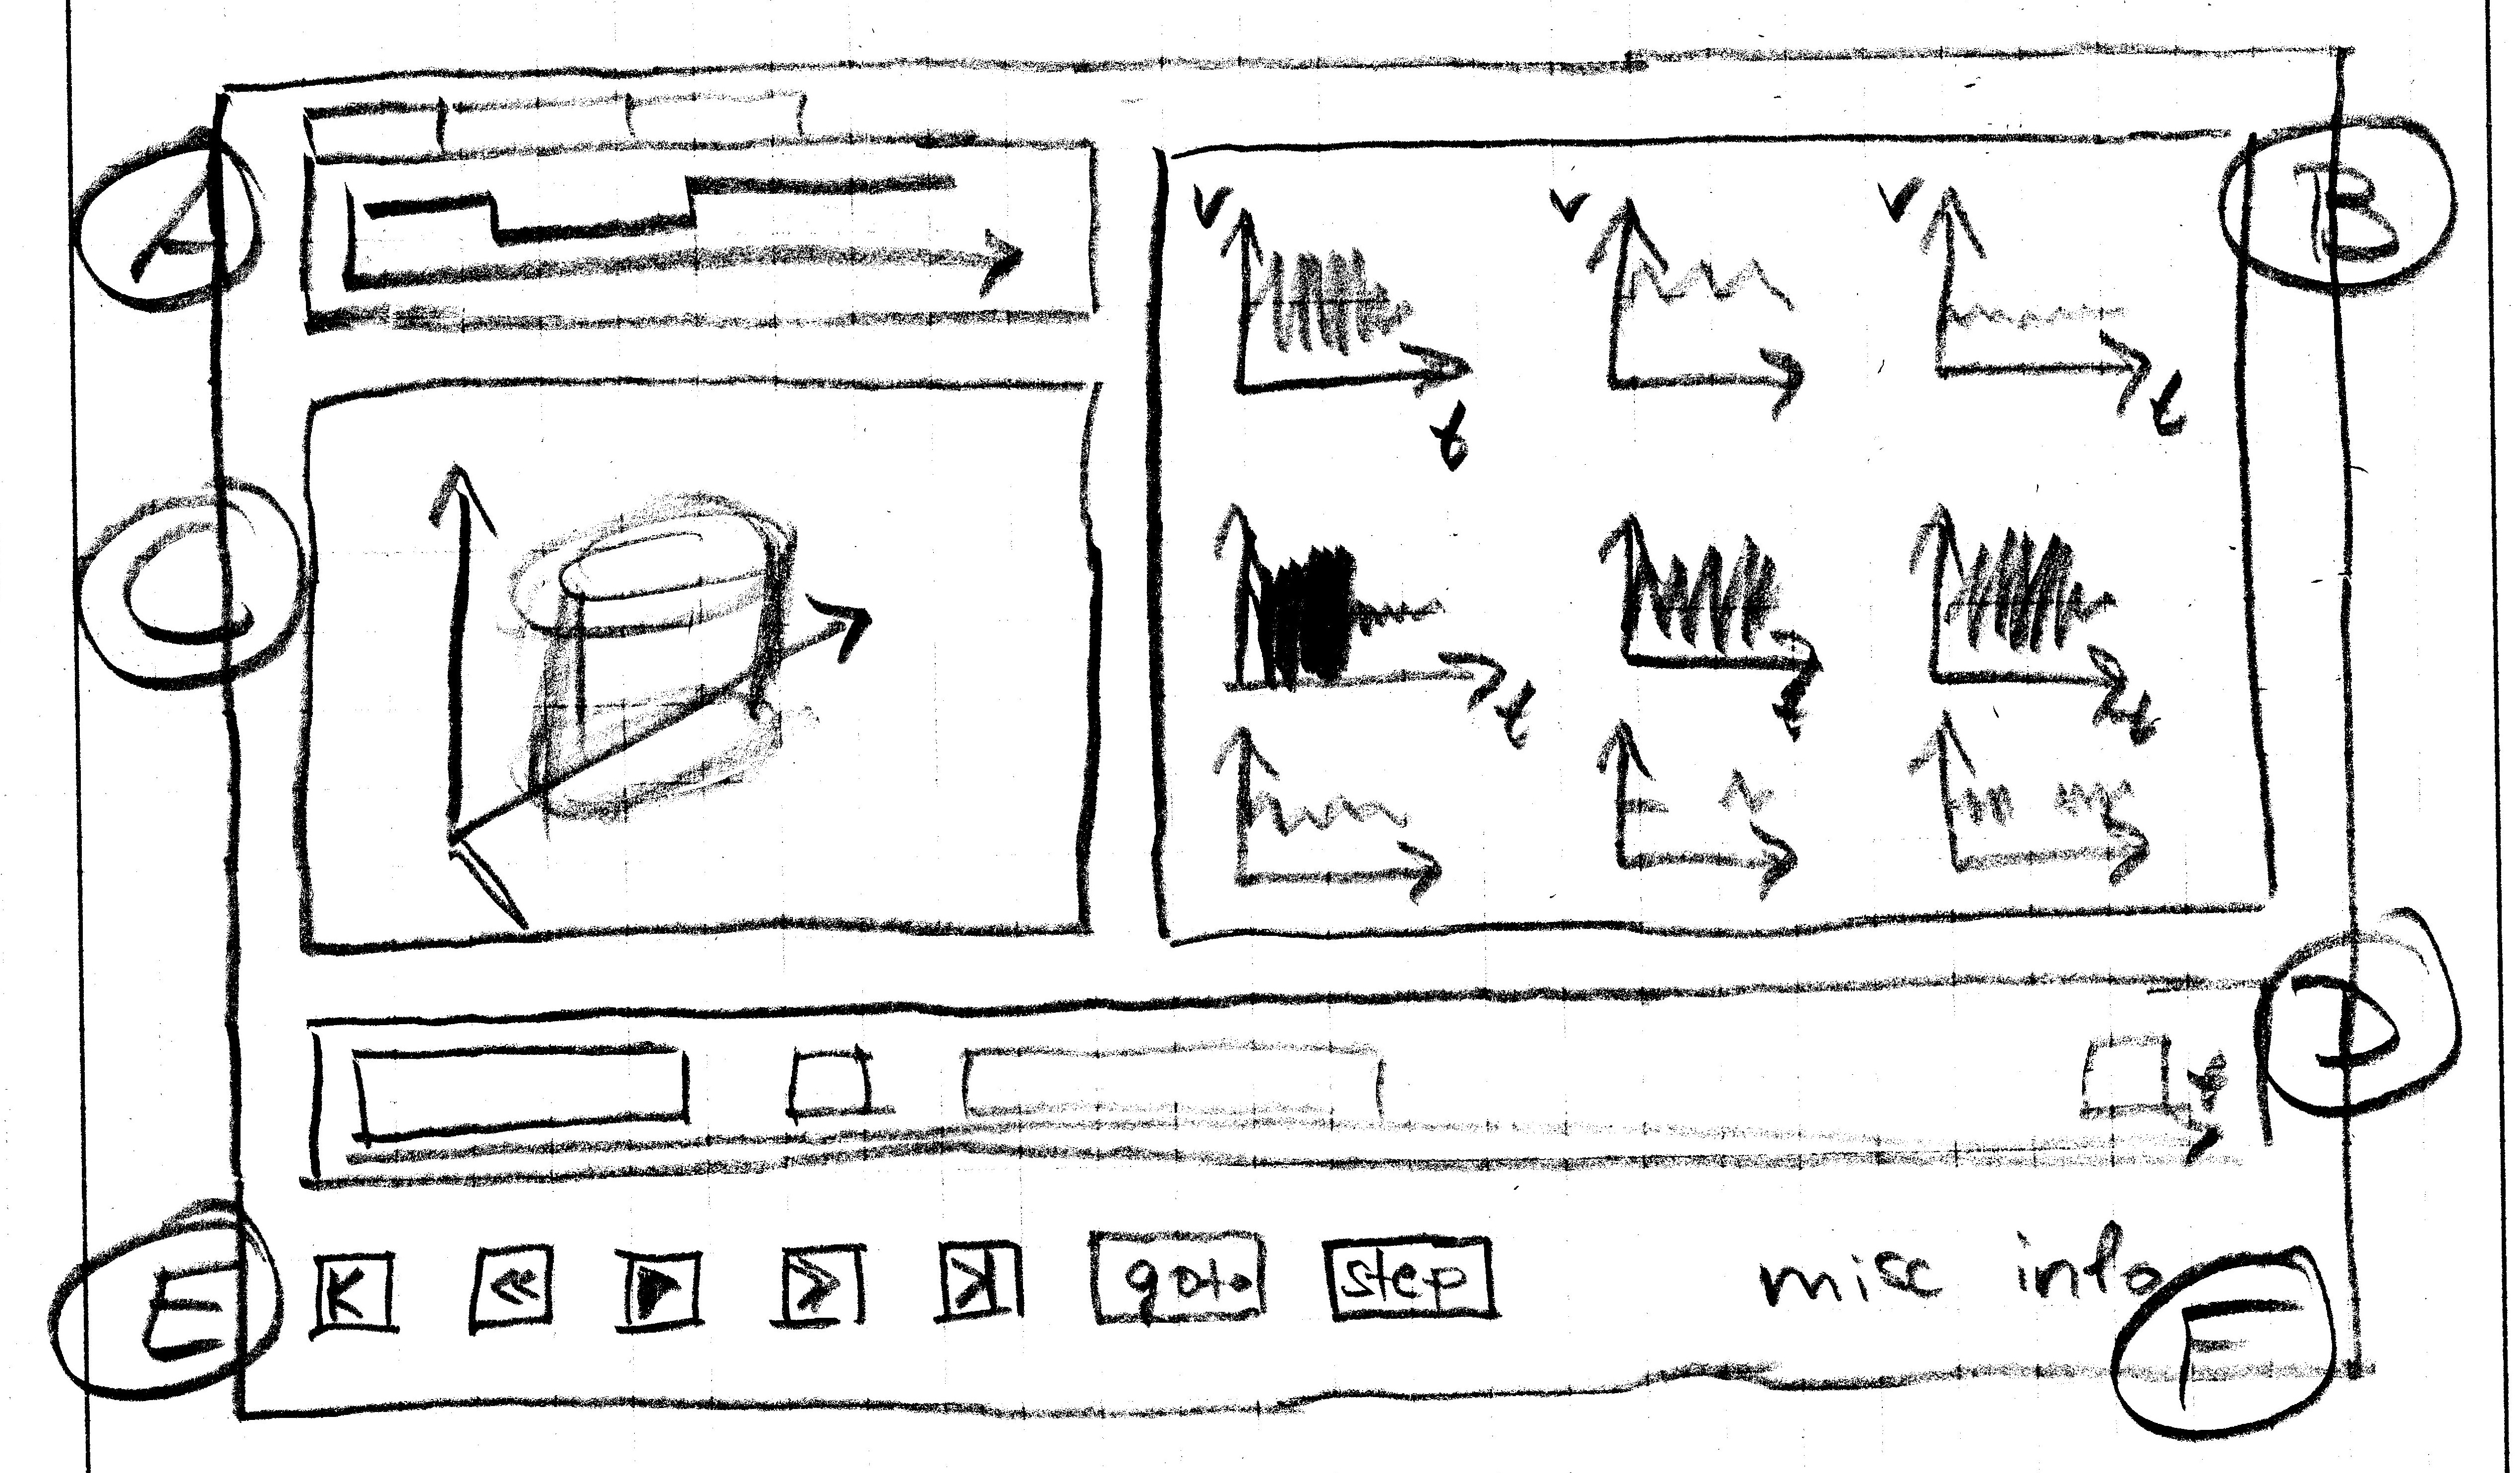
\includegraphics[width=\textwidth]{img/proto_2.jpg}
        \caption{Low-fidelity prototype view 2}
        \label{fig:lofi-2}
    \end{subfigure}%
    \\
    \begin{subfigure}{\textwidth}
        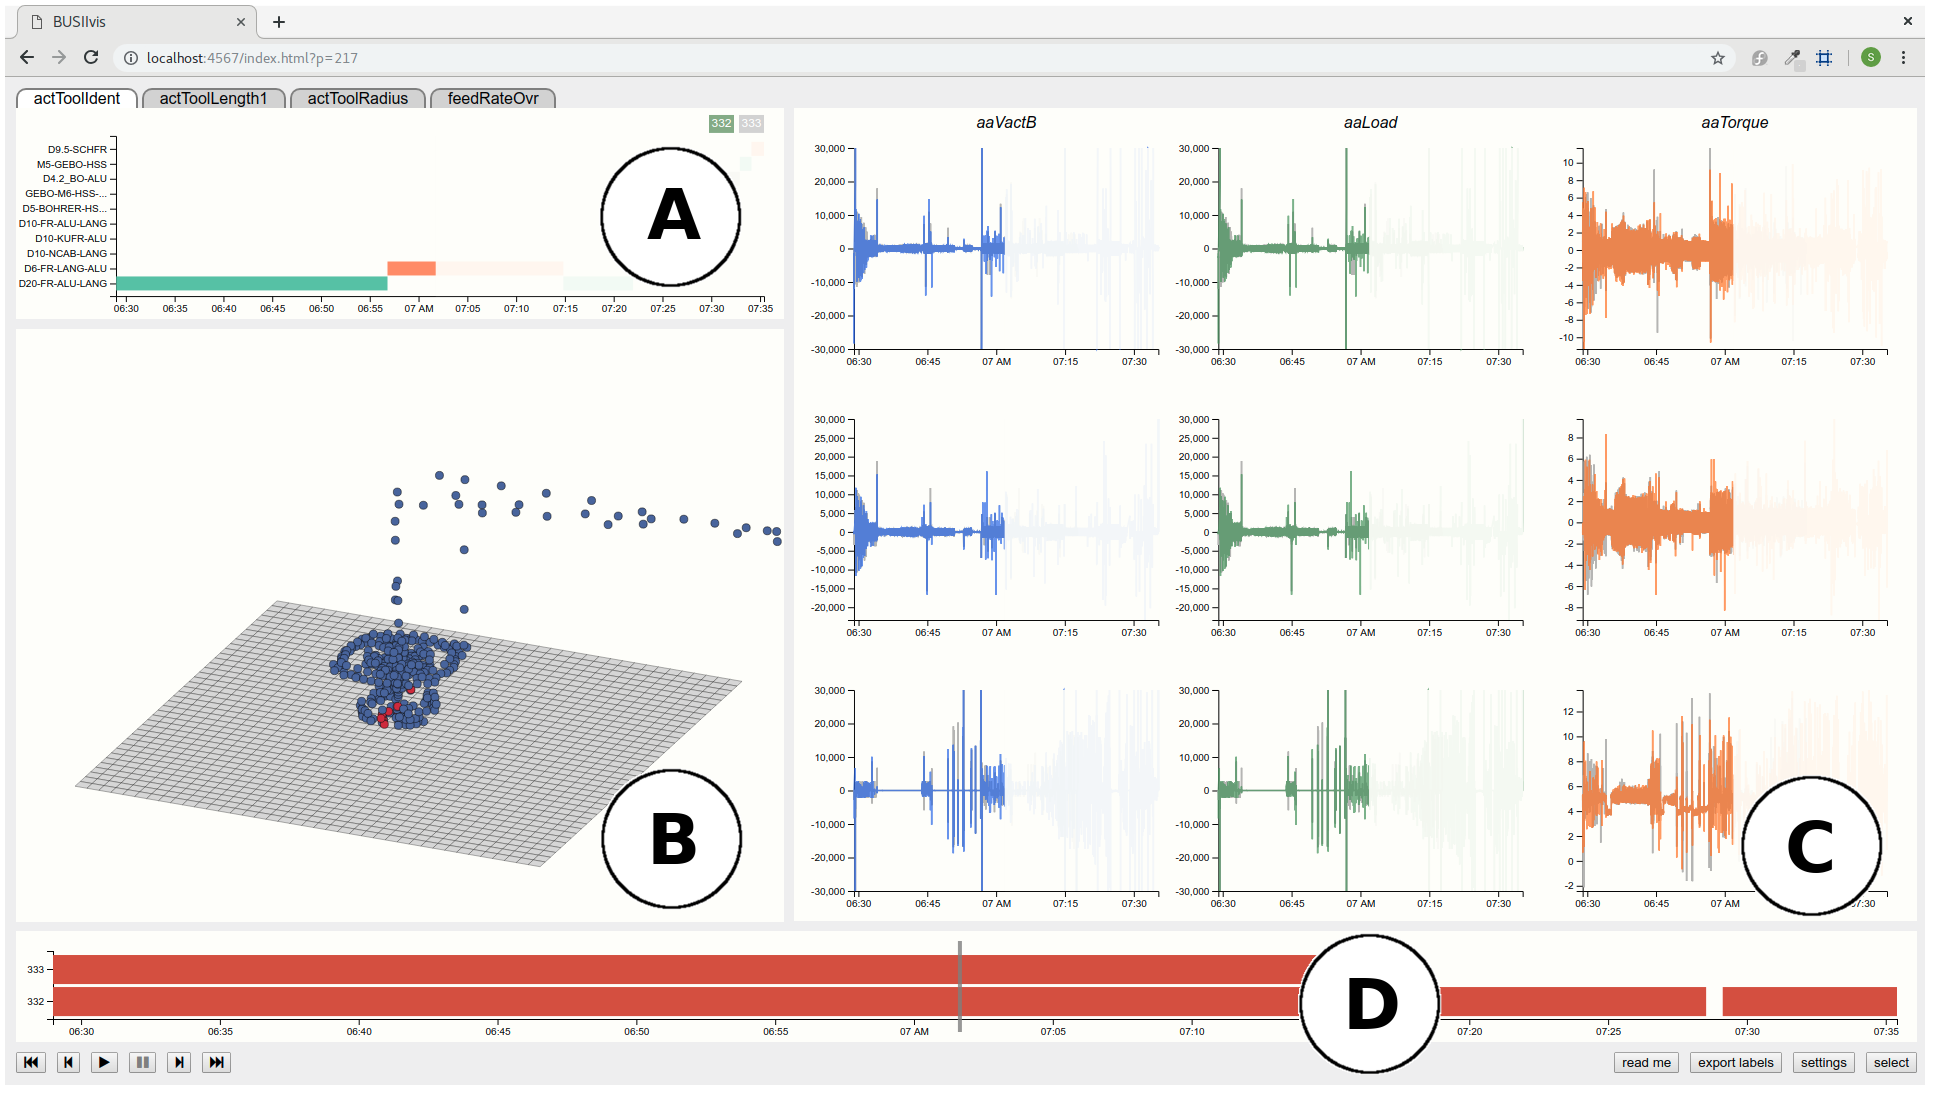
\includegraphics[width=\textwidth]{img/screen-labeled.png}
        \caption{High-fidelity prototype}
        \label{fig:hifi}
    \end{subfigure}%
    \caption{Comparison of prototypes}
\end{figure}

\begin{figure}
    \centering
    \begin{subfigure}{0.5\textwidth}
        \centering
        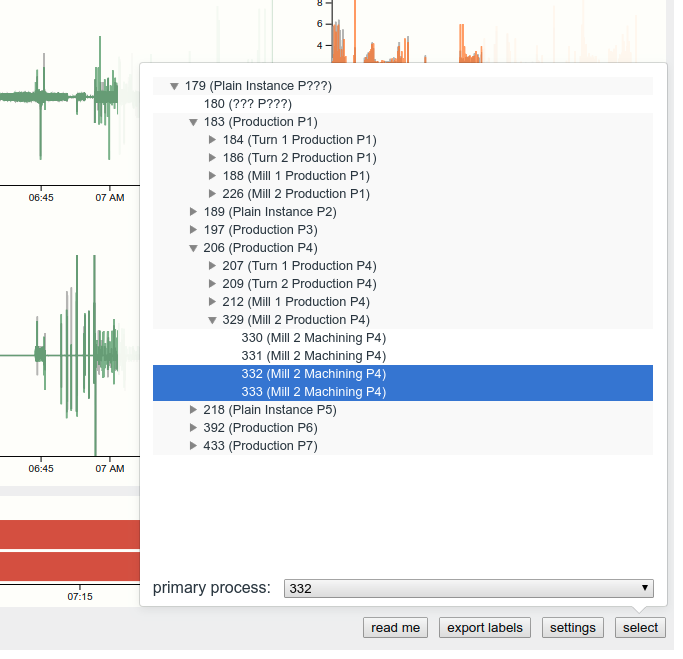
\includegraphics[width=\textwidth]{img/select.png}
        \caption{Selecting processes from the tree}
        \label{fig:select}
    \end{subfigure}%
    ~
    \begin{subfigure}{0.5\textwidth}
        \centering
        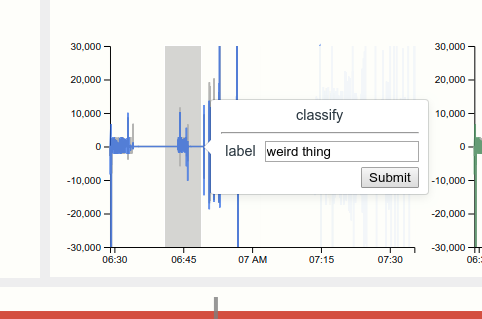
\includegraphics[width=\textwidth]{img/label-dialog.png}
        \caption{Labeling a time segment}
        \label{fig:label}
    \end{subfigure}
    \\
    \begin{subfigure}{0.5\textwidth}
        \centering
        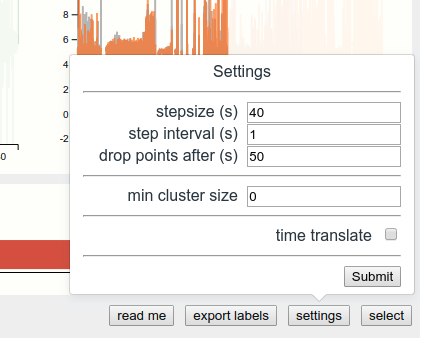
\includegraphics[width=\textwidth]{img/settings.png}
        \caption{Settings}
        \label{fig:label}
    \end{subfigure}
    \caption{UI elements}
\end{figure}

\section{Functionality}

\subsection{Description of Views}

The most important views as far as interactivity is concerned are the
activities chart (marked D in Figure~\ref{fig:hifi}) and the stepping
controls directly below it, as well as the selection and settings dialog which
can be opened by clicking the buttons at the bottom right.

The activities chart displays the time segments in which machining data was
recorded without interruptions of more than 15 seconds. It can be clicked to
update the current time step, or the vertical bar can be dragged to scan along
the time axis and update all views correspondingly. If multiple charts are selected,
they will be displayed one below the other.

The stepping controls below allow to jump to the start or the end of the
recorded events as well as (dis)enabling the automatic stepping. One single
manual step can also be taken. By default, the stepsize is calculated as
$\frac{\text{length of process}}{100}$, i.e. a process is divided into 100
steps. This can be adjusted in the settings.

The 3D scatterplot (marked B) displays the locations of the tools during the
process. The data is processed into 600 microclusters by using $k$-means to
deal with the high volume of points in some processes. Unfortunately, SVG does
not scale to thousands of elements. If more than one process are selected, the
primary process will be shown in blue and the secondary proceses in red, and
the secondary points will disappear after a predefined amount of time (by
default 10 seconds). The microclusters appear as soon as the earliest point
summarized by the cluster would have appeared.

View C shows timeseries data for the X, Y and Z axes (ordered from top to bottom).
They are not preprocessed. It might be a good idea to apply PAA (piecewise aggregate
approximation) to cut down on the number of points. Data points that would only appear
after the current timestep are hidden behind a white overlay.

A brush over the time axis can be triggered by clicking on one of the 9
timeseries charts. Right-clicking on the brush opens a dialog allowing to label
the selected segment, see Figure~\ref{fig:label}.

Finally, view A displays miscellaneous data, like the identifiers of the tools
used, their length and radius, and the feedrate override. Similar to the
timeseries view, data occuring after the current timestep are hidden behind a
white overlay. The bars of the tool identifier chart can be used to filter the
scatterplot below to display only points made by certain tools.

If multiple processes are selected, the buttons on the top right of the tool
identifier chart can be used to toggle between the processes for that chart.
The button for the primary process is green to distinguish it from the others
and to offer a visual cue as to which process is currently selected as the
primary.

\subsection{Omitted functionality}

Some functionality was omitted in the final prototype. Most notably this is the
integration of detecting discords using the Matrix Profile algorithm. Although
this algorithm is cool and potentially easy to use, it is very unclear whether
the results are meaningful---after all a time segment that is distinctly
different to all others may not necessarily be anomalous in our case. Such an
approach would be more suited for highly regular processes, e.g. a heart beat,
where deviations are clearly anomalous.

We instead spent our time implementing the option to display multiple processes
at the same time, which was suggested after the presentation of the initial
protoype, as this was deemed to be a useful feature (as opposed to integrating
MP, whose usefulness is uncertain).

\section{Implementation}

The implementation is based on the excellent SVG and DOM-manipulation library D3.
We used D3-3D for rendering 3D elements (i.e. the 3D scatterplot), which was
a bit of a hassle (the library is not very well documented, and if you have never
dealt with 3D can be a bit puzzling, and the one single example is confusing).

We have a web server which does some basic tasks such as serving the data and modifying
it, e.g. if the user wants the processes to be normalized to the same start time, it
correctly alters the timestamps, or filters out clusters that have not enough points assigned.
It also stores and aggregates the labelings done by the user.

The frontend itself is organized around some shared state including the current
time-step, which tool is currently selected (if any), and the data retrieved
from the backend. Changes triggered by the UI result in a D3 dispatcher object
being triggered, which relays the data to all views that listen to it. Thus the
views are decoupled from each other.

The data is gathered from the logs using a small army of preprocessing scripts.
Unfortunately, this takes quite a bit of time (about an hour for all
processes). Thankfully it needs to be done only once. This high time
requirement stems from data being read often (every script will read it
again---combining them would be smart) and some operations being plain costly
depending on input size, e.g. clustering many points with $k$-means.

\section{Challenges}

The main challenge was how to keep the frontend (relatively) responsive while
dealing with large amounts of data. We have made adjustments to this end
preemptively, such as microclustering the position data and summarizing
multiple data points into broken bars (i.e. activity chart).

Although the current implementation is not extremely fast and responsive, it is
very much usable without developing anger issues. The longest wait is for the
server to transfer the data (especially if time adjustments need to be made). A
further step to reduce data volume would be to use PAA to summarize points of
the timeseries data.

A big headache was to implement the possibility of comparing multiple processes after we
had already had all views and basic functionality implemented---many assumptions which
were made previously went out the window and rewriting almost all of the frontend-size
data wrangling was frustrating.

The most cumbersome and time intensive task was definitely data preparation.

\end{document}
